\chapter{Preface} 

\section*{A free and open-source calculus \ \scalebox{0.5}{\includegraphics{figures/CClicense.eps}}} 

\vspace*{-0.15in}

As we have noted in the single-variable edition of \emph{Active Calculus}, several fundamental ideas in calculus are more than 2000 years old, and calculus as a formal subdiscipline of mathematics was first introduced and developed in the late 1600s.  Mathematicians agree that the subject has been understood -- rigorously and by experts -- since the mid 1800s.  The discipline is one of our great human intellectual achievements.

While each author of a calculus textbook certainly offers her own creative perspective on the subject, it is hardly the case that many of the ideas she presents are new.  Indeed, the mathematics community broadly agrees on what the main ideas of calculus are, as well as their justification and their importance; the core parts of nearly all calculus textbooks are very similar.  As such, it is our opinion that in the 21st century -- an age where the internet permits seamless and immediate transmission of information -- no one should be required to purchase a calculus text to read, to use for a class, or to find a coherent collection of problems to solve.  Calculus belongs to humankind, not any individual author or publishing company.  Thus, a main purpose of this work is to present a new multivariable calculus text that is \emph{free}.  In addition, instructors who are looking for a multivariable calculus text should have the opportunity to download the source files and make modifications that they see fit; thus this text is \emph{open-source}.  %Since August 2013, \emph{Active Calculus} has been endorsed by the American Institute of Mathematics and its Open Textbook Initiative: \href{http://aimath.org/textbooks/}{\texttt{http://aimath.org/textbooks/}}.

Any professor or student may use an electronic version of the text for no charge.  A .pdf copy of the text may be obtained by download from the \href{http://faculty.gvsu.edu/boelkinm/Home/Active_Calculus.html}{Active Calculus home page}, or directly from
\begin{center} \href{http://gvsu.edu/s/Wb}{\texttt{http://gvsu.edu/s/Wb}}. \end{center}  
Because the text is open-source, any instructor may acquire the full set of source files, by request via email to Matt Boelkins.  

This work is licensed under the Creative Commons Attribution-NonCommercial-ShareAlike 3.0 Unported License.  The graphic 
\begin{center}
\includegraphics{figures/CClicense.eps}
\end{center}
that appears throughout the text shows that the work is licensed with the Creative Commons, that the work may be used for free by any party so long as attribution is given to the author(s), that the work and its derivatives are used in the spirit of ``share and share alike,'' and that no party may sell this work or any of its derivatives for profit.  Full details may be found by visiting
\begin{center}
\href{http://creativecommons.org/licenses/by-nc-sa/3.0/}{\texttt{http://creativecommons.org/licenses/by-nc-sa/3.0/}}
\end{center} 
or sending a letter to Creative Commons, 444 Castro Street, Suite 900, Mountain View, California, 94041, USA. 

\section*{Active Calculus - Multivariable: our goals}

In \emph{Active Calculus - Multivariable}, we endeavor to actively engage students in learning the subject through an activity-driven approach in which the vast majority of the examples are completed by students.  Where many texts present a general theory of calculus followed by substantial collections of worked examples, we instead pose problems or situations, consider possibilities, and then ask students to investigate and explore.  Following key activities or examples, the presentation normally includes some overall perspective and a brief synopsis of general trends or properties, followed by formal statements of rules or theorems.  While we often offer plausibility arguments for such results, rarely do we include formal proofs.  It is not the intent of this text for the instructor or author to \emph{demonstrate} to students that the ideas of calculus are coherent and true, but rather for students to \emph{encounter} these ideas in a supportive, leading manner that enables them to begin to understand for themselves why calculus is both coherent and true.  

This approach is consistent with the following goals:

\begin{itemize}
   \item To have students engage in an active, inquiry-driven approach, where learners strive to construct solutions and approaches to ideas on their own, with appropriate support through questions posed, hints, and guidance from the instructor and text.
   \item To build in students intuition for why the main ideas in multivariable calculus are natural and true.  We strive to accomplish this by using specific cases to highlight the ideas for the general situation using contexts that are common and familiar.
   \item To challenge students to acquire deep, personal understanding of multivariable calculus through reading the text and completing preview activities on their own, through working on activities in small groups in class, and through doing substantial exercises outside of class time.  
   \item To strengthen students' written and oral communicating skills by having them write about and explain aloud the key ideas of multivariable calculus.
\end{itemize}

\section*{Features of the Text}

Similar to the presentation of the single-variable \emph{Active Calculus}, instructors and students alike will find several consistent features in the presentation, including:

\begin{itemize}
	\item {\bf Motivating Questions.}  At the start of each section, we list \emph{motivating questions} that provide motivation for why the following material is of interest to us.  One goal of each section is to answer each of the motivating questions.
	\item {\bf Preview Activities.} Each section of the text begins with a short introduction, followed by a \emph{preview activity}.  This brief reading and the preview activity are designed to foreshadow the upcoming ideas in the remainder of the section; both the reading and preview activity are intended to be accessible to students \emph{in advance} of class, and indeed to be completed by students before a day on which a particular section is to be considered.
	\item {\bf Activities.}  Every section in the text contains several \emph{activities}.  These are designed to engage students in an inquiry-based style that encourages them to construct solutions to key examples on their own, working either individually or in small groups.  
	\item {\bf Exercises.}  There are dozens of calculus texts with (collectively) tens of thousands of exercises.  Rather than repeat standard and routine exercises in this text, we recommend the use of WeBWorK with its access to the National Problem Library and its many multivariable calculus problems.  In this text, there are a small number of challenging exercises in each section.  Almost every such exercise has multiple parts, requires the student to connect several key ideas, and expects that the student will do at least a modest amount of writing to answer the questions and explain their findings.  For instructors interested in a more conventional source of exercises, consider the freely available text by Gilbert Strang of MIT, available in .pdf format from the MIT open courseware site via \href{http://gvsu.edu/s/bh}{\texttt{http://gvsu.edu/s/bh}}.
	\item {\bf Graphics.}  As much as possible, we strive to demonstrate key fundamental ideas visually, and to encourage students to do the same.  Throughout the text, we use full-color graphics to exemplify and magnify key ideas, and to use this graphical perspective alongside both numerical and algebraic representations of calculus.  The figures and the software to generate them have been created by David Austin.
	\item {\bf Links to Java Applets.}  Many of the ideas of multivariable calculus are best understood dynamically, and there are a number of applets referenced in the text that can be used by instructors and students to assist in the investigations and demonstrations. The use of these freely available applets is in accord with our philosophy that no one should be required to purchase materials to learn calculus. We are indebted to everyone who allows their expertise to be openly shared. 
	\item {\bf Summary of Key Ideas.}  Each section concludes with a summary of the key ideas encountered in the preceding section; this summary normally reflects responses to the motivating questions that began the section.
\end{itemize}


\section*{How to Use this Text}

This text may be used as a stand-alone textbook for a standard multivariable calculus course or as a supplement to a more traditional text. 

\subsection*{Electronically}

Because students and instructors alike have access to the book in .pdf format, there are several advantages to the text over a traditional print text.  One is that the text may be projected on a screen in the classroom (or even better, on a whiteboard) and the instructor may reference ideas in the text directly, add comments or notation or features to graphs, and indeed write right on the text itself.  Students can do likewise, choosing to print only whatever portions of the text are needed for them.  In addition, the electronic version of the text includes live html links to java applets, so student and instructor alike may follow those links to additional resources that lie outside the text itself.  Finally, students can have access to a copy of the text anywhere they have an internet-enabled device.

\subsection*{Activities Workbook}

Each section of the text has a preview activity and at least three in-class activities embedded in the discussion.  As it is the expectation that students will complete all of these activities, it is ideal for them to have room to work on them adjacent to the problem statements themselves.  As a separate document, we have compiled a workbook of activities that includes only the individual activity prompts, along with space provided for students to write their responses.  This workbook is the one printing expense that students will almost certainly have to undertake, and is available upon request to the authors.  

There are also options in the source files for compiling the activities workbook with hints for each activity, or even full solutions.  These options can be engaged at the instructor's discretion.

%\subsection*{Print on Demand}

%\subsection*{Appendices}

\subsection*{Community of Users}

Because this text is free and open-source, we hope that as people use the text, they will contribute corrections, suggestions, and new material.  At this time, the best way to communicate typographical errors or suggestions for changes is by email to Matt Boelkins at \texttt{boelkinm@gvsu.edu}.  At Matt's blog, \href{http://opencalculus.wordpress.com/}{\texttt{http://opencalculus.wordpress.com/}}, we also share new developments, post feedback received by email, and include other points of discussion; readers may post additional comments and feedback.

%\subsection*{Contributors}

%The following people have generously contributed to the development or improvement of the text.  Contributing authors have written drafts of at least one; contributing editors have offered feedback, information about typographical errors, or other suggestions to improve the exposition.

%\begin{tabular}{l l l}
%\underline{Authors:} & \ & \ \\
%\ & Steven Schlicker & GVSU \\
%\ & David Austin & GVSU \\
%\ & Matt Boelkins & GVSU \\
%\underline{Contributing Editors:} & \ & \ \\
%\ & David Austin & GVSU \\
%\ & Marcia Frobish & GVSU \\
%\ & Luis Sanjuan & Conservatorio Profesional de M\'{u}sica de \'{A}vila, Spain
%\\
%\ & Steven Schlicker & GVSU \\
%\ & Jerome Trouba & Ferris State University \\
%\ & Sue Van Hattum & Contra Costa College \\
%\end{tabular}


\section*{Acknowledgments}

This text is an extension of the single variable \emph{Active Calculus} by Matt Boelkins. The initial drafts of this multivariable edition were written by Steve Schlicker; editing and revisions were made by David Austin and Matt Boelkins. David Austin is responsible for the beautiful full-color .eps graphics in the text.  Many of our colleagues at GVSU have shared their ideas and resources, which undoubtedly had a significant influence on the product. We thank them for all of their support. 

In advance, we also thank our colleagues throughout the mathematical community who will read, edit, and use this book, and hence contribute to its improvement through ongoing discussion.  

We take responsibility for all errors or inconsistencies in the text, and welcome reader and user feedback to correct them, along with other suggestions to improve the text. \\

\ \hfill David Austin, Matt Boelkins, Steven Schlicker, Allendale, MI,  July, 2015.
 
